\documentclass[12pt, a4paper]{article}
\usepackage[utf8]{inputenc}
\title{Traveling Salesman Problem}
\author{}
\usepackage[utf8]{inputenc}
\usepackage[utf8]{inputenc}
\usepackage[english]{babel}
\usepackage{hyperref}
\hypersetup{
    colorlinks=true,
    linkcolor=blue,
    filecolor=magenta,      
    urlcolor=cyan,
}
\urlstyle{same}
\usepackage{graphicx}
\usepackage{listings}
\graphicspath{ {Images/} }

\begin{document}

\vspace{3cm} 
\maketitle

\vspace{30mm} 
\centering
\large
Student : Bușe-Dragomir Alexandru

\vspace{10mm}
\centering
Artificial Intelligence, Summer 2018

\vspace{10mm}
\centering
Group I, Subgroup A

\centering
CEN 2.1A

\newpage

\vspace{20mm}
\centering
\Large 
Introduction

\vspace{30mm}
\centering
\large

\begin{flushleft}
\hspace{5mm}\textit{The travelling salesman problem (TSP) asks the following question: "Given a list of cities and the distances between each pair of cities, what is the shortest possible route that visits each city and returns to the origin city?" It is an NP-hard problem in combinatorial optimization, important in operations research and theoretical computer science.
\vspace{10mm}
\\
\hspace{5mm}The TSP has several applications even in its purest formulation, such as planning, logistics, and the manufacture of microchips. Slightly modified, it appears as a sub-problem in many areas, such as DNA sequencing. In these applications, the concept city represents, for example, customers, soldering points, or DNA fragments, and the concept distance represents travelling times or cost, or a similarity measure between DNA fragments. The TSP also appears in astronomy, as astronomers observing many sources will want to minimize the time spent moving the telescope between the sources. In many applications, additional constraints such as limited resources or time windows may be imposed. [source : Wikipedia]}
\end{flushleft}

\newpage

\vspace{30mm}
\centering
\Large 
Problem statement
\\
\vspace{2mm}
\centering
\Large 
\textit{TSP Problem}

\vspace{20mm}
\begin{flushleft}
\hspace{5mm}
\large
Travelling Salesman Problem (TSP): Given a set of cities and distance between every pair of cities, the problem is to find the shortest possible route that visits every city exactly once and returns to the starting point.
\end{flushleft}

\large
\vspace{5mm}
\begin{flushleft}
\hspace{5mm}
Your task is to develop an application to evaluate the performance of two heuristic
search algorithms.
We consider A* and Recursive best-first search – RBFS. In what follows we
present the description of RBFS:
“This algorithm uses the f limit variable to keep track of the f-value of the
best alternative path available from any ancestor of the current node. If the
current node exceeds this limit, the recursion unwinds back to the alternative
path. As the recursion unwinds, RBFS replaces the f-value of each node along
the path with a backed-up value – the best f-value of its children. In this way,
RBFS remembers the f-value of the best leaf in the forgotten subtree and can
therefore decide whether it’s worth reexpanding the subtree at some later time.”
\end{flushleft}

\vspace{10mm}
\includegraphics[scale=0.6]{numbers}
\\
\centering
\scriptsize
\vspace{2mm}

\newpage

\vspace{20mm}
\centering
\Large 
Pseudocode

\vspace{10mm}
\centering
\large
\textit{Dijkstra's Algorithm}
\vspace{10mm}

\normalsize
\begin{lstlisting}[language=Python]

// computes shortest path in a graph from source vertex
// to destination vertex


function Dijkstra(Graph, source, destination):

    create vertex priority queue Queue

    for each vertex v in Graph:              
        distance[v] <- INFINITY                  
        previous[v] <- UNDEFINED                 
        add v to Queue                       

    distance[source] <- 0                         
    
    while Queue is not empty:
        u <- vertex in Queue with min distance[u]    
                                         
        remove u from Queue 
        
        for each neighbor v of u       
            auxiliary <- distance[u] + length(u, v)
            if auxiliary < distance[v]           
                distance[v] <- auxiliary
                previous[v] <- u 

    get shortest path from dist[] and prev[]
    calculate shortest path cost
    
    return cost
\end{lstlisting}

\newpage

\centering
\large
\textit{Prim's Algorithm}
\vspace{10mm}

\normalsize
\begin{lstlisting}[language=Python]

// the code is very similar to Dijkstra
// there is only a difference in the final if


function Prim(Graph):
    
    create vertex priority queue Queue

    for each vertex v in Graph:              
        distance[v] <- INFINITY                  
        previous[v] <- UNDEFINED                 
        add v to Queue                       

    distance[source] <- 0                         
    
    while Queue is not empty
        u <- vertex in Queue with min distance[u]    
                                         
        remove u from Queue 
        
        for each neighbor v of u       
            auxiliary <- length(u, v)
            
            // differences here
            
            if auxiliary < distance[v]           
                distance[v] <- auxiliary 
                previous[v] <- u 
    
    get minimum spanning tree from dist[] and prev[]
    calculate minimum spanning tree cost
    
    return cost
    
\end{lstlisting}


\newpage
\vspace{10mm}
\centering
\Large 
Application outline

\vspace{10mm}
\centering
\large
\textit{A* class review}

\vspace{10mm}
\centering
\large

\begin{flushleft}
\hspace{5mm}
We will use in this class the following data structures and members: \\
\vspace{10mm}
\hspace{3mm}$\rightarrow$ a priority queue in which we have the nodes sorted in ascending order by their cost\\
\hspace{3mm}$\rightarrow$ a list that informs us if we have or have not already visited a certain node\\
\hspace{3mm}$\rightarrow$ a list of cities that have been visited in the visiting order to recreate the path\\
\hspace{3mm}$\rightarrow$ a total traveling cost variable to store the total cost of the chosen way\\
\hspace{3mm}$\rightarrow$ we also have a cost matrix which tells us what is the cost from vertex i to vertex j (matrix[i][j] == cost from i to j)\\
\hspace{3mm}$\rightarrow$ and a starting node which is set in the constructor of the class\\
\hspace{3mm}$\rightarrow$ this class is practically very similar with the Dijkstra class, but instead of sorting the priority queue after the edge costs, we use the total cost (i.e. the cost of the edges + heuristic cost)\\
\hspace{3mm}$\rightarrow$ implementation is using a minimum spanning tree cost from Prim's algorithm as a heuristic\\
\hspace{3mm}$\rightarrow$ implementation is using a shortest path from Dijkstra's algorithm as a heuristic\\
\end{flushleft}

\newpage
\centering
\large
\textit{A* solve method}

\vspace{5mm}
\begin{flushleft}
\hspace{3mm}$\rightarrow$ we are in the initial town at the start, so we mark it as visited and we add it to the visitedNodes list\\
\hspace{3mm}$\rightarrow$ we save in a variable the total number of visited nodes, initially 1\\
\hspace{3mm}$\rightarrow$ we visit nodes until all nodes (cities) have been visited\\
\hspace{3mm}$\rightarrow$ we take each node, except the current one, and check if it is visited; we don't have to check if there is an edge from one to another because the graph is complete\\
\hspace{3mm}$\rightarrow$ we take all neighbours (we do not have self loops); we check if the neighbours are visited or not\\
\hspace{3mm}$\rightarrow$ for each neighbour which is not visited, we calculate the totalCost with one of the two heuristics, using a Minimum Spanning Tree (Prim's Algorithm) or a shortest path (Dijkstra's Algorithm)\\
\hspace{3mm}$\rightarrow$ for each neighbour which is not visited, we calculate the totalCost we get the total cost on the edges of the spanning tree and save it; this is the heuristic value for the current node\\
\hspace{3mm}$\rightarrow$ we calculate the total cost by adding the heuristic cost and the cost on the edge to this node\\
\hspace{3mm}$\rightarrow$ now we create the node and we save it in the priorityQueue\\
\hspace{3mm}$\rightarrow$ in other words, like in the case of Dijkstra algorithm, we add in the priority queue all the neighbours of the current node which are not visited\\
\hspace{3mm}$\rightarrow$ now we update the currentNode and mark it as visited and then we add it to the visitedNodes list; increase visitedNodesNumber\\
\hspace{3mm}$\rightarrow$ now we update the currentNode and mark it as visited and then we add it to the visitedNodes list; increase visitedNodesNumber\\
\hspace{3mm}$\rightarrow$ we get the total cost of the tour for the travel trough all nodes\\
\end{flushleft}

\centering
\large
\textit{RBFS class review}

\vspace{10mm}
\centering
\large

\begin{flushleft}
\hspace{5mm}
We will use in this class the following data structures and members: \\
\vspace{10mm}
\hspace{3mm}$\rightarrow$ implementation of recursive best first search; is using Prim's and Dijkstra's algorithms as heuristics (cost of minimum spanning tree and shortest path cost)\\
\hspace{3mm}$\rightarrow$ a priority queue in which we have the nodes sorted in ascending order by their cost\\
\hspace{3mm}$\rightarrow$ a list that informs us if we have or have not already visited a certain node\\
\hspace{3mm}$\rightarrow$ a list of cities that have been visited in the visiting order to recreate the path\\
\hspace{3mm}$\rightarrow$ a total traveling cost variable to store the total cost of the chosen way\\
\hspace{3mm}$\rightarrow$ we also have a cost matrix which tells us what is the cost from vertex i to vertex j (matrix[i][j] == cost from i to j)\\
\hspace{3mm}$\rightarrow$ and a starting node which is set in the constructor of the class\\
\hspace{3mm}$\rightarrow$ this class is practically very similar with the A* class, but instead of sorting the priority queue after the cost of the edges + heuristic cost, we use only the heuristic cost\\
\hspace{3mm}$\rightarrow$ implementation is using a minimum spanning tree cost from Prim's algorithm as a heuristic\\
\hspace{3mm}$\rightarrow$ implementation is using a shortest path from Dijkstra's algorithm as a heuristic\\
\end{flushleft}

\newpage
\centering
\large
\textit{RBFS solve method}

\vspace{5mm}
\begin{flushleft}
\hspace{3mm}$\rightarrow$ we will save information in the ArrayLists from the position 1 in order to logically retrieve information from them because the cities have indices from 1 to "numberOfNodes"\\

\hspace{3mm}$\rightarrow$ we initialise the isVisited list with false; the traveling cost will be 0 at the start of the tour\\

\hspace{3mm}$\rightarrow$ function returns true if we found a way to visit nodes at a new level; returning false means that we must go back; the final path can be recreated by seeing the content of the visitedNodes\\

\hspace{3mm}$\rightarrow$ we save in a variable the total number of visited nodes, initially 1; we have this in an if because we want to initialise it only once, in the first call of the recursive function\\

\hspace{3mm}$\rightarrow$ if we are in the point in which we know that the tour was found, we must get out of the recursion (we went trough all the nodes of the graph)\\

\hspace{3mm}$\rightarrow$ the current node is marked as visited because we are working with it; we go trough all neighbours of the current node except the node itself\\

\hspace{3mm}$\rightarrow$ we apply Dijkstra/Prim algorithms to the graph (only the unvisited nodes)\\

\hspace{3mm}$\rightarrow$ we retrieve the heuristic cost - the cost of all the edges of the shortest path; final cost = edge cost + heuristic cost\\

\hspace{3mm}$\rightarrow$ we create a node object for the neighbour and we add it to the queue\\

\hspace{3mm}$\rightarrow$ while we can go down into the recursion, we search for a path; algorithm goes back if we find a bad heuristic and we unwind to get to the second best node which is upper in the search graph; each return from the recursion gets up a level in the search, because each new recursion goes to the neighbours of a node, so "deeper"\\

\newpage
\hspace{3mm}$\rightarrow$ we use peek method which gives us the top node from the queue without removing it from the queue; we also save the index of this node\\

\hspace{3mm}$\rightarrow$ if the heuristic value of the main node is worst that the fLimit, then we must go back and choose the alternative node (second minimum)\\

\hspace{3mm}$\rightarrow$ we update the costs while going back to all parents of the node which had a worse fLimit, until we reach the alternative; we mark the current node as unvisited because it is no longer a good option\\

\hspace{3mm}$\rightarrow$ in order not to modify the original pQueue, we save it into an auxiliary one; we remove the top value and peek the other one (we get the second smallest value); this is the alternative node (we return here depending on the fLimit value)\\

\hspace{3mm}$\rightarrow$ then we check if the neighbour with the minimum cost is good; if so, we go deeper in the recursion (one level down); if the neighbour represents a good option, we add it to the visited list; we mark it as visited; we continue to search trough its neighbours\\

\hspace{3mm}$\rightarrow$ else, we can't go any further, it's a dead end, so we go back; on the way back, we update the heuristic value; we mark the current node as unvisited because it is no longer a good option; \\

\hspace{3mm}$\rightarrow$ we get the total cost of the tour for the travel trough all nodes; we iterate trough the visitedNodes list and sum the costs of the path; we get from costMatrix the cost for adjacent edges and add them\\
\end{flushleft}

\newpage
\centering
\large
Overview of the classes
\vspace{20mm}
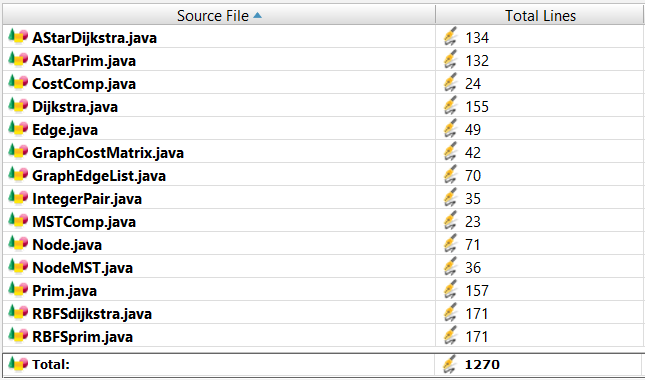
\includegraphics{Image1.PNG}
\vspace{20mm}
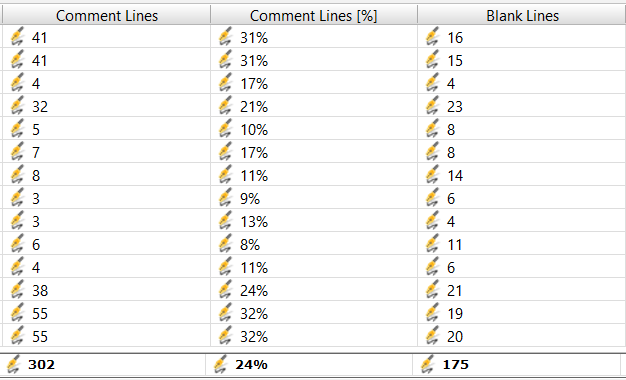
\includegraphics{Image2.PNG}

\newpage
\vspace{10mm}
\centering
\large 
Experiments and results

\normalsize
\vspace{10mm}
\begin{flushleft}

\hspace{5mm}In order to generate the input tests, I used a function that asks for the number of vertices (we will call it v) in the graph and the maximum cost per one edge (we will call it max) and outputs in a file a matrix with v rows and v columns.\\
\vspace{3mm}
\hspace{5mm} So matrix[x][y] = cost of edge from x to y and also matrix[x][x] = 0; we consider that we have an edge between any two nodes, so v(v-1)/2 edges, the matrix being symmetric. \\
\vspace{3mm}
\hspace{5mm} To sum up, we have a matrix[v+1][v+1] (storing nodes from index 1) and matrix[i][j] has a value of [1..max] if i != j or 0 if i == j.

\vspace{5mm}
\scriptsize
\begin{lstlisting}

/// generates edges with values between 1 and maxCostPerEdge
/// they are saved in a costMatrix and then copied in an output file
/// in order not to have a stack overflow, I restricted the number of vertices to 100

void generateNodes(int numberOfNodes, int maxCostPerEdge)
{
    int costOfEdge = 0;
    int costMatrix[101][101] = {0};

    srand(time(NULL));

    for(int row = 1; row <= numberOfNodes; row ++)
    {
        for(int column = 1; column <= numberOfNodes; column ++)
        {
            if(row < column)
            {
                costOfEdge = rand() % maxCostPerEdge + 1;

                costMatrix[row][column] = costOfEdge;

                costMatrix[column][row] = costOfEdge;
            }
        }
    }

    for(int row = 1; row <= numberOfNodes; row ++)
    {
        for(int column = 1; column <= numberOfNodes; column ++)
        {
            file << costMatrix[row][column] << " ";
        }

        file << '\n';
    }

    file.close();
}

\end{lstlisting}
\end{flushleft}

\newpage
\vspace{25mm}
\centering
\large 
Conclusions

\small
\vspace{30mm}
\begin{flushleft}

\hspace{5mm}For me, the implementation of this project has been an opportunity to test my level of preparation regarding the Artificial Intelligence object and the degree in which I can apply my Java and C++ language knowledge in solving problems which are bound to this area of study.
\\
\vspace{3mm}
\hspace{5mm}At the same time, it was a good way to improve my methods of processing and editing documents in LaTeX. I also understood the importance of having a well structured project documentation which does include a well organized source code, programs for testing the main application, non-trivial inputs etc.
\\
\vspace{3mm}
\hspace{5mm}It was a good exercise of correct code indentation, documentation, object oriented programming, design, algorithmic thinking and mathematics.
\\
\vspace{3mm}
\hspace{5mm}I enjoyed developing the source code and analyzing the situations that arose in the process because these have shown me once more the undeniable link that connects mathematics, algorithms and programming, creating the fundamentals of Artificial Intelligence.
\\
\vspace{3mm}
\hspace{5mm}I will finish by saying that the process of assembling all the project parts into one application has represented a very good practice for my long term growth associated to the domain of programming.

\end{flushleft}

\newpage
\vspace{10mm}
\centering
\large 
References

\vspace{20mm}
\scriptsize
\begin{lstlisting}

1.http://software.ucv.ro/~cbadica/ai/cap6.pdf

2.http://ieor.berkeley.edu/~aaswani/teaching/FA13/151/lecture_notes/ieor151_lec17.pdf

3.http://www1.cse.wustl.edu/~ychen/7102/Karp-TSP.pdf

4.https://courses.cs.washington.edu/courses/csep521/01au/lectures/lecture2slides.pdf

5.https://www.geeksforgeeks.org/travelling-salesman-problem-set-2-approximate-using-mst/

6.https://www.geeksforgeeks.org/greedy-algorithms-set-5-prims-minimum-spanning-tree-mst-2/

7.https://www.geeksforgeeks.org/greedy-algorithms-set-6-dijkstras-shortest-path-algorithm/

8.https://en.wikipedia.org/wiki/Minimum_spanning_tree

9.https://stackoverflow.com/questions/1909281/use-dijkstras-to-find-a-minimum-spanning-tree

10.http://auajournal.uab.ro/upload/48_611_Pop-Zelina.pdf

11.https://stackoverflow.com/questions/4453477/using-a-to-solve-travelling-salesman

12.https://www.eecs.yorku.ca/course_archive/2013-14/F/3401/slides/15b-RBFS.pdf

13. http://www.iosrjournals.org/iosr-jce/papers/Vol10-issue5/R0105105110.pdf

\end{lstlisting}

\end{document}
